% This is LLNCS.DEM the demonstration file of
% the LaTeX macro package from Springer-Verlag
% for Lecture Notes in Computer Science,
% version 2.4 for LaTeX2e as of 16. April 2010
%
\documentclass{llncs}
%
\usepackage{makeidx}  % allows for indexgeneration
\usepackage{url}
\usepackage{graphicx}
%
\begin{document}
%
\frontmatter          % for the preliminaries
%
\pagestyle{headings}  % switches on printing of running heads
%
\mainmatter              % start of the contributions
%
\title{Media Meets Semantic Web \newline How the BBC uses DBpedia and Linked Data \newline to Make Connections}
%
\titlerunning{Media Meets Semantic Web}  % abbreviated title (for running head), also used for the TOC unless \toctitle is used
%
\author{Andreas M\"{u}ller}
%
\authorrunning{Andreas M\"{u}ller} % abbreviated author list (for running head)
%
%%%% list of authors for the TOC (use if author list has to be modified)
\tocauthor{Andreas M\"{u}ller}
%
\institute{Technische Universit\"{a}t Berlin, 10623, Germany,\\
  \email{andreas.mueller.4@campus.tu-berlin.de},\\ WWW home page:
  \texttt{\url{http://www.user.tu-berlin.de/hpdesigner_20}}
}

\maketitle              % typeset the title of the contribution

\begin{abstract} % 70-150 words
This paper describes, how the BBC managed to better interlink different BBC domains by introducing DBpedia as a common vocabulary for every domain. Given the existing legacy systems, the BBC was already using, it is shown, how the new Semantic Web technology was integrated and used, to interlink documents and providing a better usability and user experience, allowing the user to browse different BBC domains by following a semantic thread and getting cross-domain information.
\keywords{linked data, semantic web, bbc, dbpedia}
\end{abstract}
%
\section{Introduction}
%
The British Broadcasting Corporation (BBC) is the oldest and still one of the largest Broadcasting Companies in the world. Given the fact, that the BBC is producing online content since 1994 \cite{st1994}, they have a huge amount of online media content today in text, audio and video format. To make the data accessible, it was categorized and organized in different domains, i.e. news, sport, weather etc. Figure \ref{fig:domains2009} and \ref{fig:domains2017} present these domains the way they were displayed on the BBC website in the years 2009 and 2017. Each domain became a separate microsite with its own content, vocabulary and datasets.
\begin{figure}[!ht]
  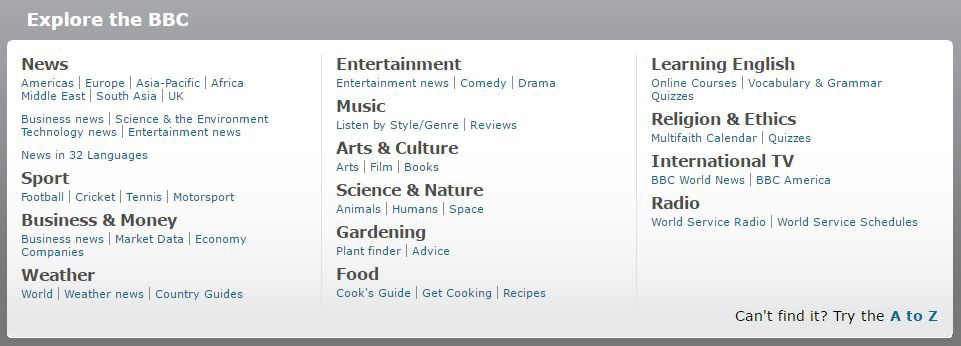
\includegraphics[width=\textwidth]{images/bbc_domains_2009}
  \caption{BBC microsites in June, 2009}
  \label{fig:domains2009}
\end{figure}
\begin{figure}[!ht]
  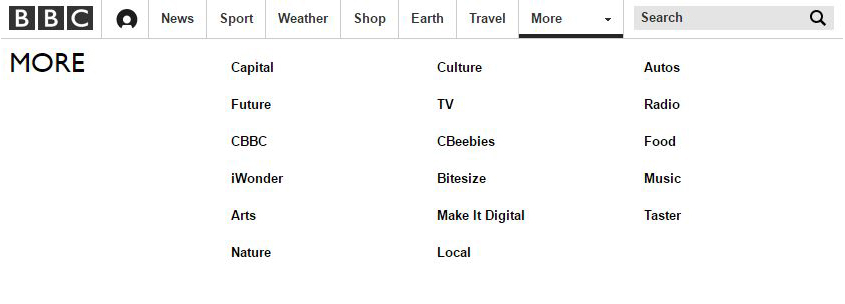
\includegraphics[width=\textwidth]{images/bbc_domains_2017}
  \caption{BBC microsites in June, 2017}
  \label{fig:domains2017}
\end{figure}

This separation of content created a clear structure where the user instantly knew where to navigate to when he searched for content of a particular domain. But it also came with a big disadvantage: It was neither possible to find everything, the BBC has published to a given subject nor to navigate between different BBC domains following a semantic thread (i.e. on a page about a musician was no possibility to see all programmes that played this artist). The reason for this lack of interoperability was the missing interlinking between the different microsites. Without this interlinking, the real potential of the available data was not used.

\vspace{15mm}

To make the BBC website more coherent and more useful, G.Kobilarov et al. proposed a solution \cite{mmsw} with the following objectives:
\begin{enumerate}
  \item Build better connections and interlinking of existing systems
  \item Reducing impact on existing systems while adding new services to maximize interlinking of domains
\end{enumerate}

The next section will give a short overview of the existing legacy systems of the BBC website.

\section{Background}
%
\begin{figure}[!h]
  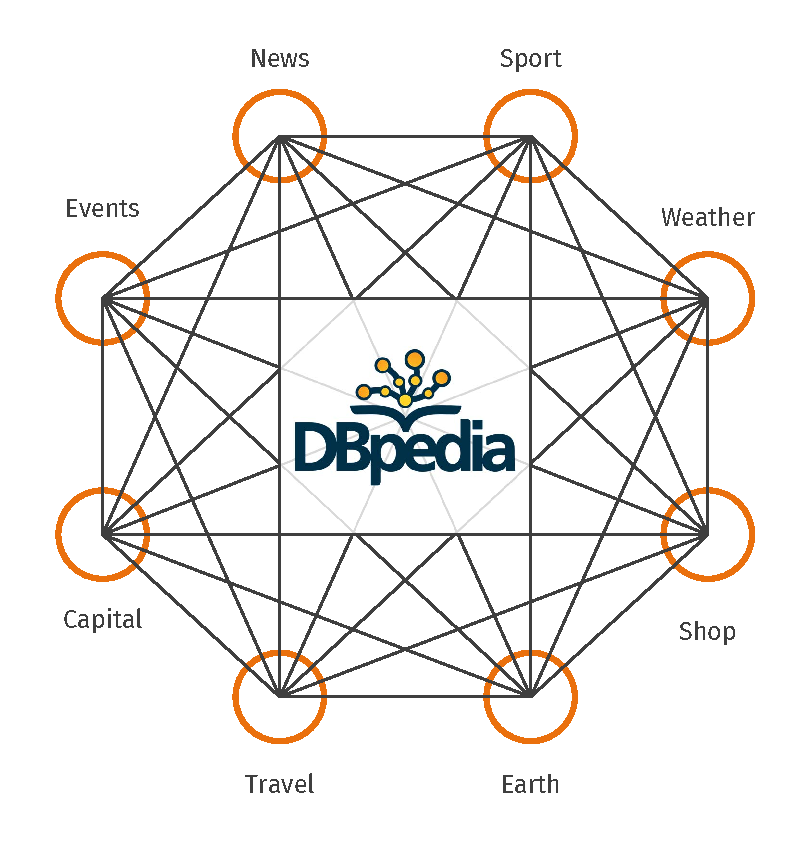
\includegraphics[width=\textwidth]{images/dbpedia_dark}
  \caption{BBC microsites connected by DBpedia}
  \label{fig:dbpedia}
\end{figure}
%
\section{Solution}
%
\begin{figure}[!h]
  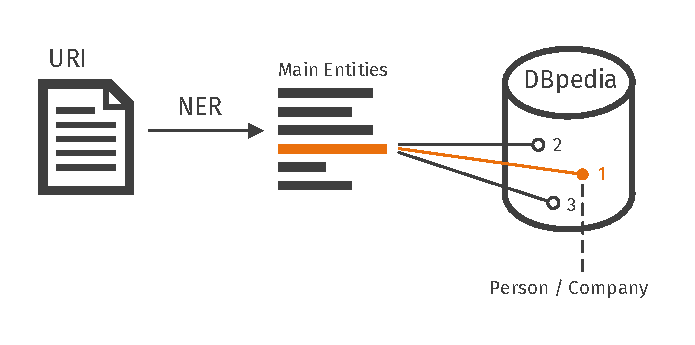
\includegraphics[width=\textwidth]{images/muddy_boots_dark}
  \caption{Muddy Boots}
  \label{fig:muddy}
\end{figure}
%
\section{Evaluation}
%
...
%
\section{Related Work}
%
...
%
\section{Future Work \& conclusions}
%
...

%
% \subsection{Autonomous Systems}
%
% \begin{figure}
% \vspace{2.5cm}
% \caption{This is the caption of the figure displaying a white eagle and
% a white horse on a snow field}
% \end{figure}
%
% \paragraph{Notes and Comments.}
% The results in this section are a
% refined version of \cite{clar:eke};
% the minimality result of Proposition
% 14 was the first of its kind.

% \begin{table}
% \caption{This is the example table taken out of {\it The
% \TeX{}book,} p.\,246}
% \begin{center}
% \begin{tabular}{r@{\quad}rl}
% \hline
% \multicolumn{1}{l}{\rule{0pt}{12pt}
%                    Year}&\multicolumn{2}{l}{World population}\\[2pt]
% \hline\rule{0pt}{12pt}
% 8000 B.C.  &     5,000,000& \\
%   50 A.D.  &   200,000,000& \\
% 1650 A.D.  &   500,000,000& \\
% 1945 A.D.  & 2,300,000,000& \\
% 1980 A.D.  & 4,400,000,000& \\[2pt]
% \hline
% \end{tabular}
% \end{center}
% \end{table}
%

%
% ---- Bibliography ----
%
\begin{thebibliography}{5}
%
\bibitem {mmsw}
  G.Kobilarov, T.Scott,Y .Raimond, S.Oliver, C.Sizemore, M.Smethurst, C.Bizer and R.Lee.:
  \textit{Media meets semantic web - How the bbc uses dbpedia and linked data to make connections}.
  Lecture Notes in Computer Science (including subseries Lecture Notes in Artificial Intelligence and Lecture Notes in Bioinformatics)
  5554LNCS:723–737, 2009.
%
\bibitem {st1994}
  The Sunday Times:
  \textit{THE BBC is launching an on-line service}. 17 April 1994.
  Quoted in Connor, Alan (25 December 2007). "The WWW Info-Rainforest". \textit{BBC Internet Blog}. BBC.

\end{thebibliography}

\end{document}
